\documentclass[10pt,
% a4paper,
%twocolumn,
fleqn,
%landscape, 
% papersize,
dvipdfmx,
uplatex
]{jsarticle}



\def\maru#1{\textcircled{\scriptsize#1}}%丸囲み番号

% \RequirePackage[2020/09/30]{platexrelease}

%太字設定
\usepackage[deluxe]{otf}

\usepackage{emathEy}

\usepackage[g]{esvect}

%大きな文字
\usepackage{fix-cm}

%定理環境
\usepackage{emathThm}
%\theoremstyle{boxed}
\theorembodyfont{\normalfont}
\newtheorem{Question}{問題}[subsection]
\newtheorem{Q}{}[subsection]
\newtheorem{question}[Question]{}
\newtheorem{quuestion}{}[subsection]

%セクション,大問番号のデザイン
\renewcommand{\labelenumi}{(\arabic{enumi})}
\renewcommand{\theenumii}{\alph{enumii})}
\renewcommand{\thesection}{第\arabic{section}章}

%用紙サイズの詳細設定
\usepackage{bxpapersize}
\papersizesetup{size={80mm,45mm}}
\usepackage[top=0.7zw,bottom=0truemm,left=3truemm,right=133truemm]{geometry}
\usepackage[dvipdfmx]{graphicx}

%余白など
\usepackage{setspace} % 行間
\setlength{\mathindent}{1zw}
\setlength\parindent{0pt}


%色カラーに関する設定
\usepackage{color}
\definecolor{shiro}{rgb}{0.95703125,0.87109375,0.7421875}
\definecolor{kin}{rgb}{0.95703125,0.87109375,0.7421875}
\definecolor{orange}{rgb}{1,0.7,0.2}
\definecolor{bradorange}{rgb}{1,0.5,0}
\definecolor{pink}{rgb}{0.9176,0.5686,0.5960}
\definecolor{mizu}{rgb}{0.6156,0.8,0.9955}
\color{kin}
% \pagecolor{hukamido}

\usepackage{at}%図の配置
% \usepackage{wallpaper}

\begin{document}



\at(0cm,0cm){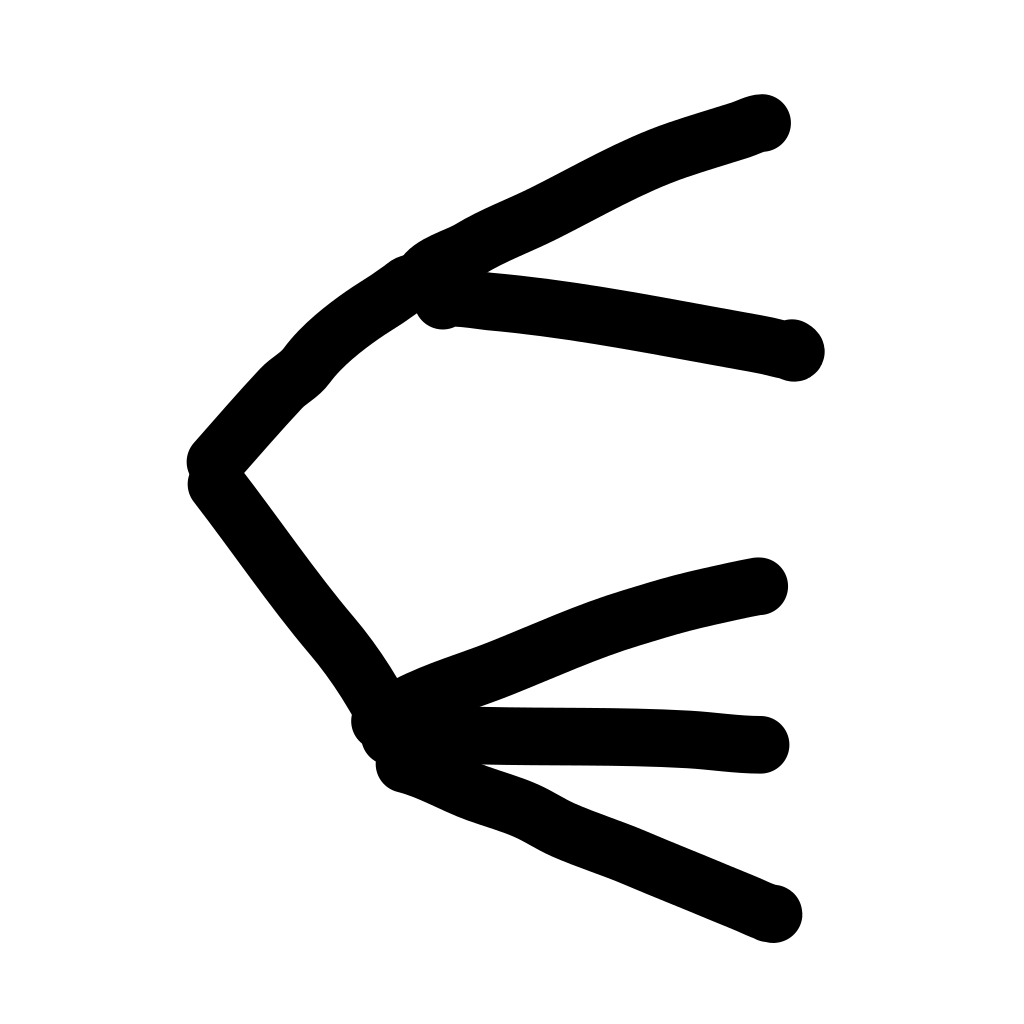
\includegraphics[width=8cm,bb=0 0 1920 1080]{./youtube/thumbnails/templates/smart_background/場合の数.jpeg}}
{\color{orange}\bf\boldmath\LARGE\underline{同じものを含む順列}}\vspace{0.3zw}

\large
\bf\boldmath 問.6つの文字

\Huge
\vspace{-0.2zw}
% \hspace{0.2zw}
A,\;A,\;A,\;B,\;B,\;C\vspace{-0.2zw}\\
\hfill を$1$列に並べる方法
\vspace{0.1zw}

\large
\hfill
は何通りか.
\at(7.0cm,0.2cm){\small\color{bradorange}$\overset{\text{場合の数}}{\text{基本}}$}


\newpage



\at(0cm,0cm){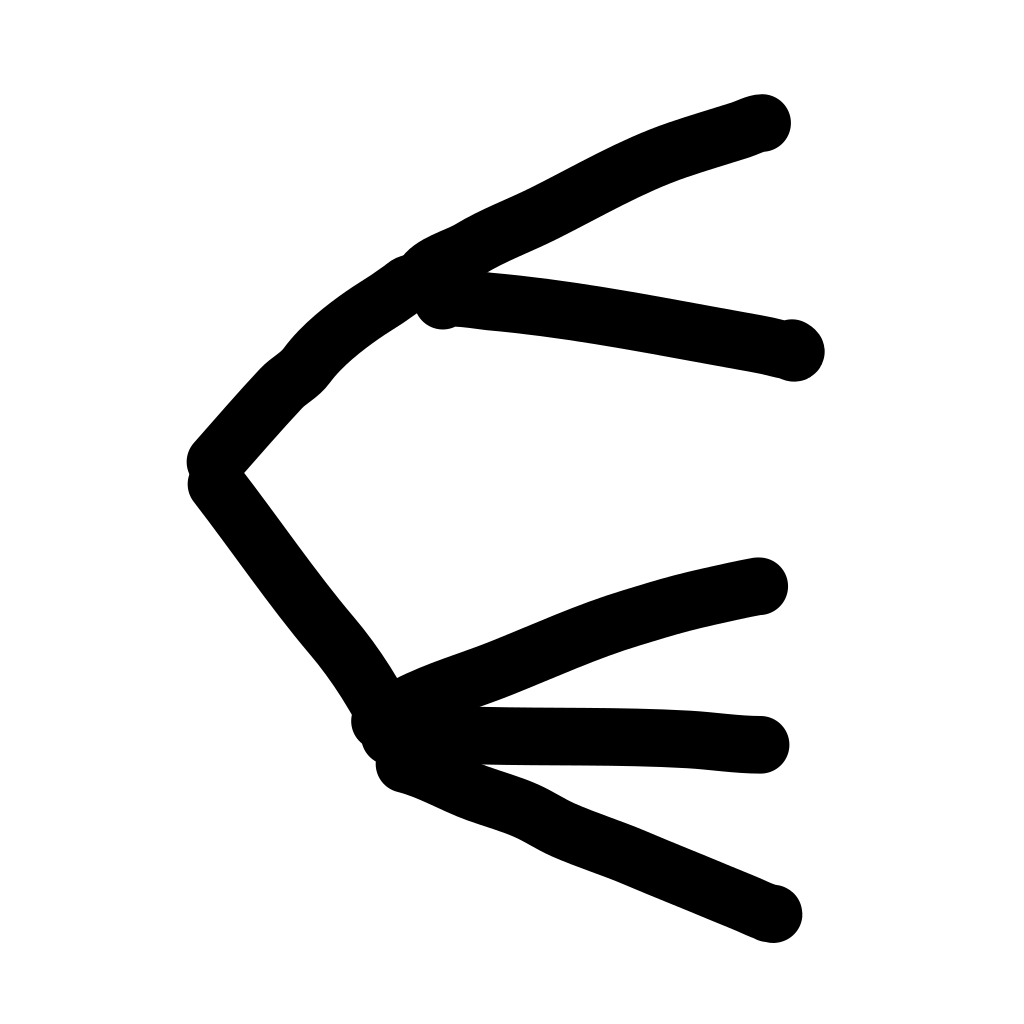
\includegraphics[width=8cm,bb=0 0 1920 1080]{./youtube/thumbnails/templates/smart_background/場合の数.jpeg}}
{\color{orange}\bf\boldmath\huge\underline{組合せ}}\vspace{0.3zw}

\large
\bf\boldmath 問.5つの文字

\huge
\vspace{-0.2zw}
A,\;B,\;C,\;D,\;E から\\
\hfill $3$つを選んで作る組合せ
\vspace{0.1zw}

\large
\hfill
は何通りか.
\at(7.0cm,0.2cm){\small\color{bradorange}$\overset{\text{場合の数}}{\text{基本}}$}


\newpage



\at(0cm,0cm){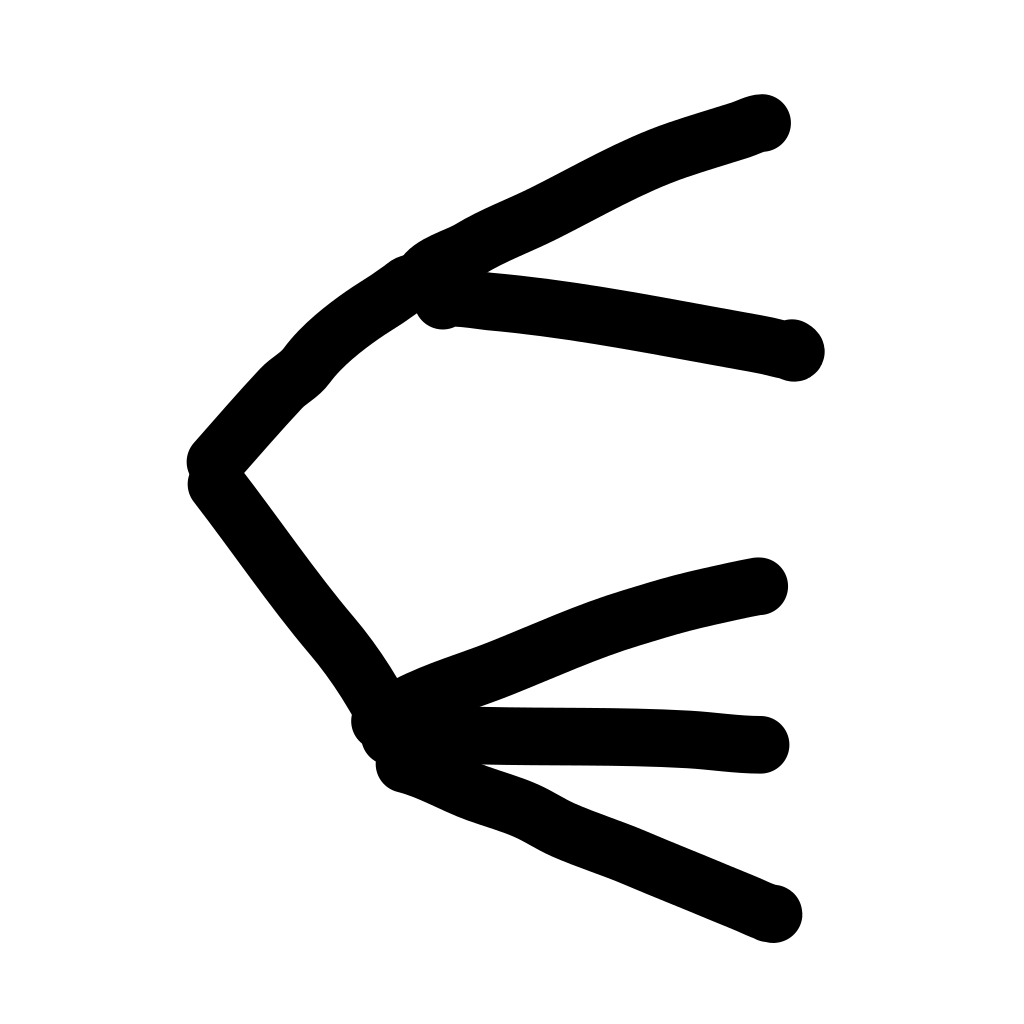
\includegraphics[width=8cm,bb=0 0 1920 1080]{./youtube/thumbnails/templates/smart_background/場合の数.jpeg}}
{\color{orange}\bf\boldmath\huge\underline{数珠順列}}\vspace{0.3zw}

\large
\bf\boldmath 問.5つの文字が描かれた玉

\huge
\vspace{-0.2zw}
A,\;B,\;C,\;D,\;E を\\
\hfill 使って数珠を作る方法
\vspace{0.1zw}

\large
\hfill
は何通りか.
\at(7.0cm,0.2cm){\small\color{bradorange}$\overset{\text{場合の数}}{\text{基本}}$}


\newpage



\at(0cm,0cm){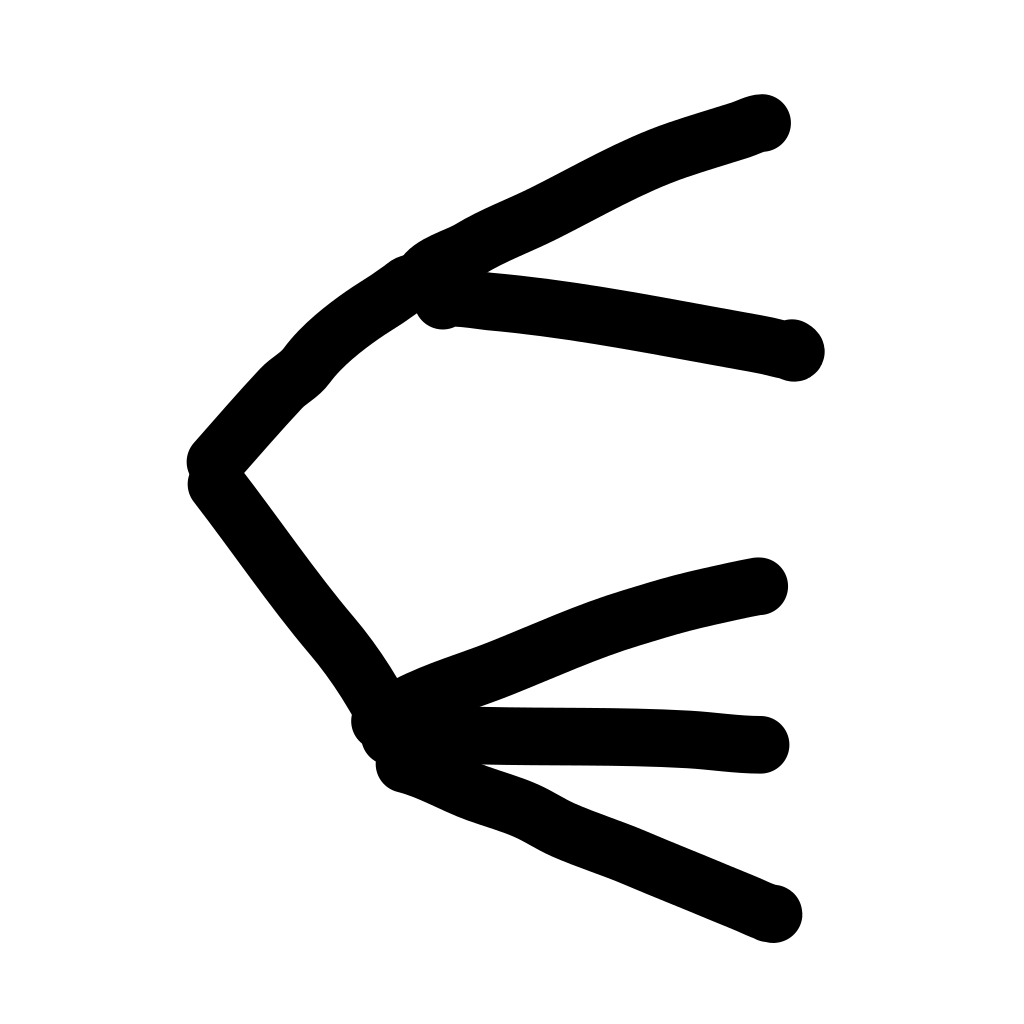
\includegraphics[width=8cm,bb=0 0 1920 1080]{./youtube/thumbnails/templates/smart_background/場合の数.jpeg}}
{\color{orange}\bf\boldmath\huge\underline{円順列}}\vspace{0.3zw}


\large
\bf\boldmath 問.5つの文字

\Huge
\vspace{-0.2zw}
A,\;B,\;C,\;D,\;E を\vspace{-0.2zw}\\
\hfill 
円形に並べる方法
\vspace{0.1zw}

\large
\hfill
は何通りか.
\at(7.0cm,0.2cm){\small\color{bradorange}$\overset{\text{場合の数}}{\text{基本}}$}


\newpage



\at(0cm,0cm){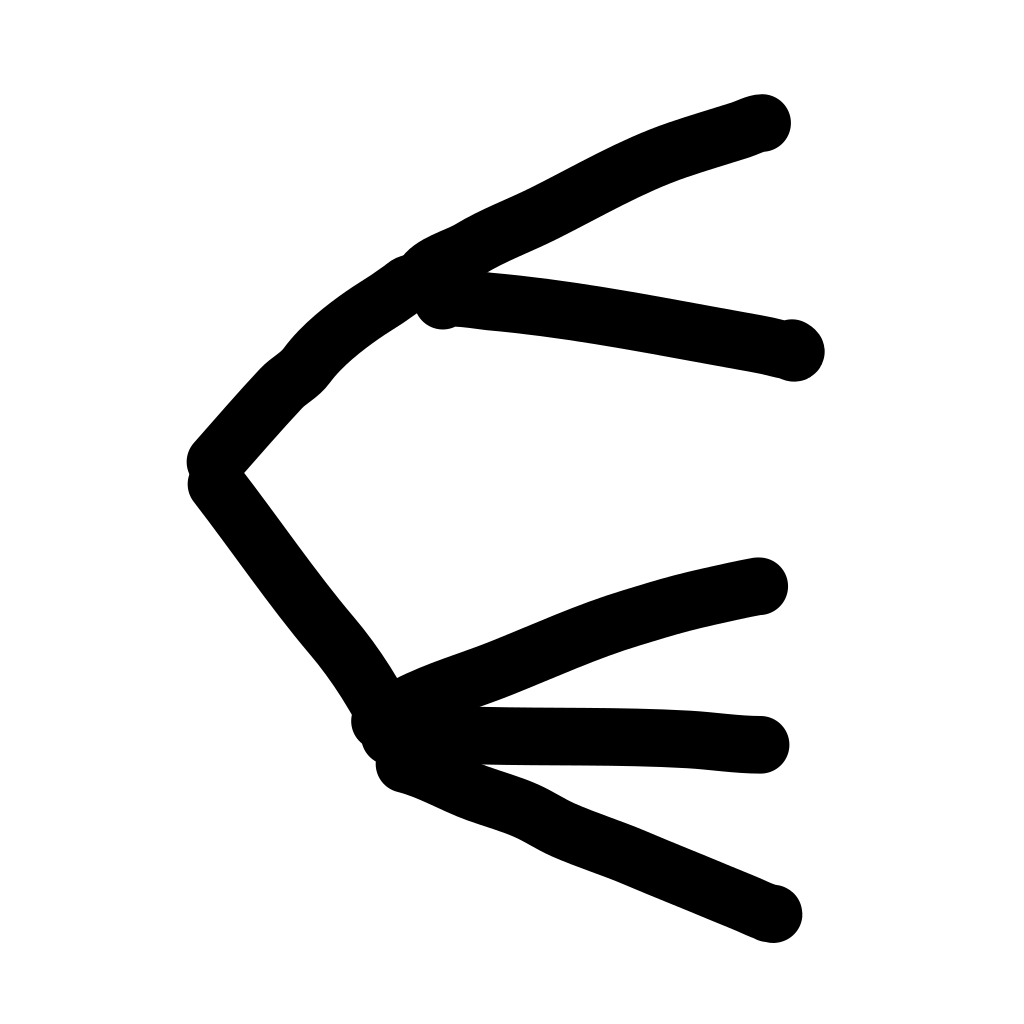
\includegraphics[width=8cm,bb=0 0 1920 1080]{./youtube/thumbnails/templates/smart_background/場合の数.jpeg}}
{\color{orange}\bf\boldmath\huge\underline{選んで並べる順列}}\vspace{0.3zw}

\large
\bf\boldmath 問.5つの文字

\huge
\vspace{-0.2zw}
A,\;B,\;C,\;D,\;Eから\\
\hfill $3$つを選んで並べる方法
\vspace{0.1zw}

\large
\hfill
は何通りか.
\at(7.0cm,0.2cm){\small\color{bradorange}$\overset{\text{場合の数}}{\text{基本}}$}


\newpage



\at(0cm,0cm){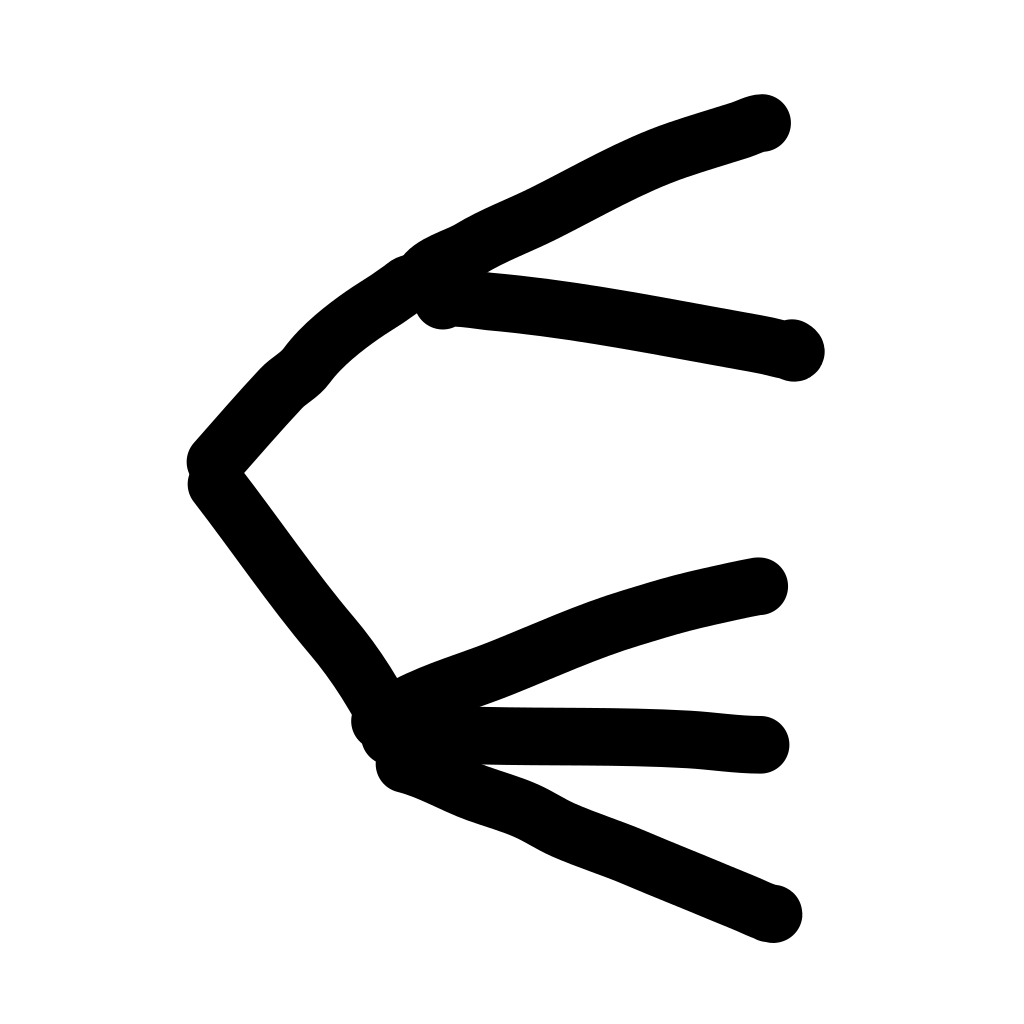
\includegraphics[width=8cm,bb=0 0 1920 1080]{./youtube/thumbnails/templates/smart_background/場合の数.jpeg}}
{\color{orange}\bf\boldmath\huge\underline{すべて並べる順列}}\vspace{0.3zw}

\large
\bf\boldmath 問.4つの文字

\Huge
\vspace{-0.2zw}
A,\;B,\;C,\;Dを\vspace{-0.2zw}\\
\hfill $1$列に並べる方法
\vspace{0.1zw}

\large
\hfill
は何通りか.
\at(7.0cm,0.2cm){\small\color{bradorange}$\overset{\text{場合の数}}{\text{基本}}$}


\end{document}

